% Auto-generated by paper/scripts/generate_figures.py
% figure-bounds width=128 height=76
\begingroup
\scriptsize
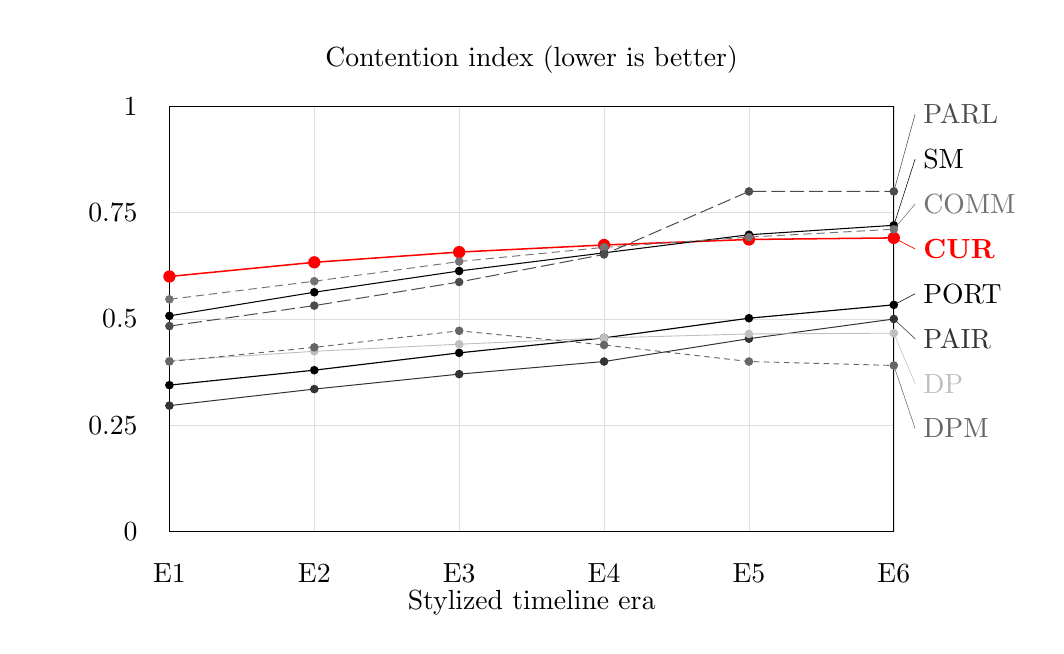
\begin{tikzpicture}[x=1mm,y=1mm]
\path[use as bounding box] (0,0) rectangle (128.0,76.0);
\draw[black!13,line width=0.18pt] (18.0,12.0) -- (110.0,12.0);
\node[anchor=east] at (15.2,12.0) {0};
\draw[black!13,line width=0.18pt] (18.0,25.5) -- (110.0,25.5);
\node[anchor=east] at (15.2,25.5) {0.25};
\draw[black!13,line width=0.18pt] (18.0,39.0) -- (110.0,39.0);
\node[anchor=east] at (15.2,39.0) {0.5};
\draw[black!13,line width=0.18pt] (18.0,52.5) -- (110.0,52.5);
\node[anchor=east] at (15.2,52.5) {0.75};
\draw[black!13,line width=0.18pt] (18.0,66.0) -- (110.0,66.0);
\node[anchor=east] at (15.2,66.0) {1};
\draw[black!12,line width=0.18pt] (18.0,12.0) -- (18.0,66.0);
\node[anchor=north] at (18.0,9.2) {E1};
\draw[black!12,line width=0.18pt] (36.4,12.0) -- (36.4,66.0);
\node[anchor=north] at (36.4,9.2) {E2};
\draw[black!12,line width=0.18pt] (54.8,12.0) -- (54.8,66.0);
\node[anchor=north] at (54.8,9.2) {E3};
\draw[black!12,line width=0.18pt] (73.2,12.0) -- (73.2,66.0);
\node[anchor=north] at (73.2,9.2) {E4};
\draw[black!12,line width=0.18pt] (91.6,12.0) -- (91.6,66.0);
\node[anchor=north] at (91.6,9.2) {E5};
\draw[black!12,line width=0.18pt] (110.0,12.0) -- (110.0,66.0);
\node[anchor=north] at (110.0,9.2) {E6};
\draw[black,line width=0.28pt] (18.0,12.0) rectangle (110.0,66.0);
\draw[red,line width=0.55pt] (18.0,44.4) -- (36.4,46.2) -- (54.8,47.5) -- (73.2,48.4) -- (91.6,49.1) -- (110.0,49.3);
\fill[red] (18.0,44.4) circle[radius=0.78];
\fill[red] (36.4,46.2) circle[radius=0.78];
\fill[red] (54.8,47.5) circle[radius=0.78];
\fill[red] (73.2,48.4) circle[radius=0.78];
\fill[red] (91.6,49.1) circle[radius=0.78];
\fill[red] (110.0,49.3) circle[radius=0.78];
\draw[black,line width=0.38pt] (18.0,39.4) -- (36.4,42.4) -- (54.8,45.1) -- (73.2,47.4) -- (91.6,49.7) -- (110.0,50.9);
\fill[black] (18.0,39.4) circle[radius=0.55];
\fill[black] (36.4,42.4) circle[radius=0.55];
\fill[black] (54.8,45.1) circle[radius=0.55];
\fill[black] (73.2,47.4) circle[radius=0.55];
\fill[black] (91.6,49.7) circle[radius=0.55];
\fill[black] (110.0,50.9) circle[radius=0.55];
\draw[black!55,line width=0.34pt,dash pattern=on 3pt off 1.8pt] (18.0,41.5) -- (36.4,43.8) -- (54.8,46.3) -- (73.2,48.1) -- (91.6,49.4) -- (110.0,50.4);
\fill[black!55] (18.0,41.5) circle[radius=0.55];
\fill[black!55] (36.4,43.8) circle[radius=0.55];
\fill[black!55] (54.8,46.3) circle[radius=0.55];
\fill[black!55] (73.2,48.1) circle[radius=0.55];
\fill[black!55] (91.6,49.4) circle[radius=0.55];
\fill[black!55] (110.0,50.4) circle[radius=0.55];
\draw[black!70,line width=0.36pt,dash pattern=on 5pt off 1.8pt] (18.0,38.1) -- (36.4,40.7) -- (54.8,43.7) -- (73.2,47.2) -- (91.6,55.2) -- (110.0,55.2);
\fill[black!70] (18.0,38.1) circle[radius=0.55];
\fill[black!70] (36.4,40.7) circle[radius=0.55];
\fill[black!70] (54.8,43.7) circle[radius=0.55];
\fill[black!70] (73.2,47.2) circle[radius=0.55];
\fill[black!70] (91.6,55.2) circle[radius=0.55];
\fill[black!70] (110.0,55.2) circle[radius=0.55];
\draw[black!80,line width=0.36pt] (18.0,28.0) -- (36.4,30.1) -- (54.8,32.0) -- (73.2,33.6) -- (91.6,36.5) -- (110.0,39.0);
\fill[black!80] (18.0,28.0) circle[radius=0.55];
\fill[black!80] (36.4,30.1) circle[radius=0.55];
\fill[black!80] (54.8,32.0) circle[radius=0.55];
\fill[black!80] (73.2,33.6) circle[radius=0.55];
\fill[black!80] (91.6,36.5) circle[radius=0.55];
\fill[black!80] (110.0,39.0) circle[radius=0.55];
\draw[black,line width=0.42pt] (18.0,30.6) -- (36.4,32.5) -- (54.8,34.7) -- (73.2,36.6) -- (91.6,39.1) -- (110.0,40.8);
\fill[black] (18.0,30.6) circle[radius=0.55];
\fill[black] (36.4,32.5) circle[radius=0.55];
\fill[black] (54.8,34.7) circle[radius=0.55];
\fill[black] (73.2,36.6) circle[radius=0.55];
\fill[black] (91.6,39.1) circle[radius=0.55];
\fill[black] (110.0,40.8) circle[radius=0.55];
\draw[black!25,line width=0.32pt] (18.0,33.7) -- (36.4,34.9) -- (54.8,35.8) -- (73.2,36.6) -- (91.6,37.1) -- (110.0,37.2);
\fill[black!25] (18.0,33.7) circle[radius=0.55];
\fill[black!25] (36.4,34.9) circle[radius=0.55];
\fill[black!25] (54.8,35.8) circle[radius=0.55];
\fill[black!25] (73.2,36.6) circle[radius=0.55];
\fill[black!25] (91.6,37.1) circle[radius=0.55];
\fill[black!25] (110.0,37.2) circle[radius=0.55];
\draw[black!60,line width=0.34pt,dash pattern=on 2pt off 1.6pt] (18.0,33.6) -- (36.4,35.4) -- (54.8,37.5) -- (73.2,35.7) -- (91.6,33.6) -- (110.0,33.1);
\fill[black!60] (18.0,33.6) circle[radius=0.55];
\fill[black!60] (36.4,35.4) circle[radius=0.55];
\fill[black!60] (54.8,37.5) circle[radius=0.55];
\fill[black!60] (73.2,35.7) circle[radius=0.55];
\fill[black!60] (91.6,33.6) circle[radius=0.55];
\fill[black!60] (110.0,33.1) circle[radius=0.55];
\draw[black!60,line width=0.2pt] (110.0,33.1) -- (112.7,25.1);
% legend-label label=DPM x=113.5 y=25.1
\node[anchor=west,inner sep=0.5pt,text=black!60] at (113.5,25.1) {DPM};
\draw[black!25,line width=0.2pt] (110.0,37.2) -- (112.7,30.8);
% legend-label label=DP x=113.5 y=30.8
\node[anchor=west,inner sep=0.5pt,text=black!25] at (113.5,30.8) {DP};
\draw[black!80,line width=0.2pt] (110.0,39.0) -- (112.7,36.5);
% legend-label label=PAIR x=113.5 y=36.5
\node[anchor=west,inner sep=0.5pt,text=black!80] at (113.5,36.5) {PAIR};
\draw[black,line width=0.2pt] (110.0,40.8) -- (112.7,42.2);
% legend-label label=PORT x=113.5 y=42.2
\node[anchor=west,inner sep=0.5pt,text=black] at (113.5,42.2) {PORT};
\draw[red,line width=0.25pt] (110.0,49.3) -- (112.7,47.9);
% legend-label label=CUR x=113.5 y=47.9
\node[anchor=west,inner sep=0.5pt,text=red] at (113.5,47.9) {\textbf{CUR}};
\draw[black!55,line width=0.2pt] (110.0,50.4) -- (112.7,53.6);
% legend-label label=COMM x=113.5 y=53.6
\node[anchor=west,inner sep=0.5pt,text=black!55] at (113.5,53.6) {COMM};
\draw[black,line width=0.2pt] (110.0,50.9) -- (112.7,59.3);
% legend-label label=SM x=113.5 y=59.3
\node[anchor=west,inner sep=0.5pt,text=black] at (113.5,59.3) {SM};
\draw[black!70,line width=0.2pt] (110.0,55.2) -- (112.7,65.0);
% legend-label label=PARL x=113.5 y=65.0
\node[anchor=west,inner sep=0.5pt,text=black!70] at (113.5,65.0) {PARL};
\node at (64.0,3.0) {Stylized timeline era};
\node[anchor=south] at (64.0,69.0) {Contention index (lower is better)};
\end{tikzpicture}
\endgroup
